\documentclass[12pt]{article}

\usepackage{fontspec}
\newfontfamily\handwriting{a-casual-handwritten-pen}[Path=../assets/fonts/,Extension=.ttf,Scale=1.5]
\newfontfamily\comic{Comic Neue}

\usepackage[utf8]{inputenc}
\usepackage{amsmath}
\usepackage{amssymb}
\usepackage{enumitem}
\usepackage{xcolor}
\usepackage{soul}
\usepackage{tikz}
\usepackage[most]{tcolorbox}
\usepackage{titlesec}
\usepackage{multicol}
\usepackage{environ}

\usetikzlibrary{fit, positioning, arrows.meta}

% --- Custom Colors ---
\definecolor{primaryblue}{RGB}{42, 111, 151}
\definecolor{exbg}{RGB}{255, 240, 245}
\definecolor{rulebg}{RGB}{232, 245, 233}
\definecolor{highlight}{RGB}{255, 243, 176}
\definecolor{pinkanno}{RGB}{255, 105, 180}
\definecolor{purpleanno}{RGB}{147, 112, 219}
\definecolor{solutionbg}{RGB}{245, 245, 255}

% --- Header Styling ---
\titleformat{\section}{\color{primaryblue}\normalfont\Large\bfseries}{\thesection}{1em}{}
\titleformat{\subsection}{\color{primaryblue}\normalfont\large\bfseries}{\thesubsection}{1em}{}

% --- Friendly Boxes ---
% --- Auto-numbered Example Box ---
\newcounter{examplenum}

\newtcolorbox{friendlyexbox}[1]{
    colback=exbg,
    colframe=pinkanno!50,
    arc=5pt,
    title=\textbf{#1},
    coltitle=black,
    attach title to upper,
    after title={:\quad}
}

\newenvironment{friendlyex}{%
    \refstepcounter{examplenum}%
    \begin{friendlyexbox}{Example \theexamplenum}%
}{%
    \end{friendlyexbox}%
}

\newtcolorbox{friendlyrule}[1]{
    colback=rulebg,
    colframe=primaryblue!30,
    arc=5pt,
    fonttitle=\bfseries,
    title={#1},
    coltitle=primaryblue
}

\newcommand{\funhl}[1]{\sethlcolor{highlight}\hl{#1}}

% --- Show/Hide Solutions ---
\newif\ifshowsolutions

% Uncomment the next line to show solutions.
\showsolutionstrue

\newcommand{\solutionblank}{\vspace{25ex}}

\NewEnviron{solutionbox}{
\ifshowsolutions
\begin{tcolorbox}[
    colback=solutionbg,
    colframe=purpleanno!45,
    arc=5pt,
    title={Solution},
    coltitle=primaryblue,
    fonttitle=\bfseries
]
\BODY
\end{tcolorbox}
\else
\solutionblank
\fi
}

% --- Coordinate Grid Command ---
\newcommand{\blankgrid}{
\begin{center}
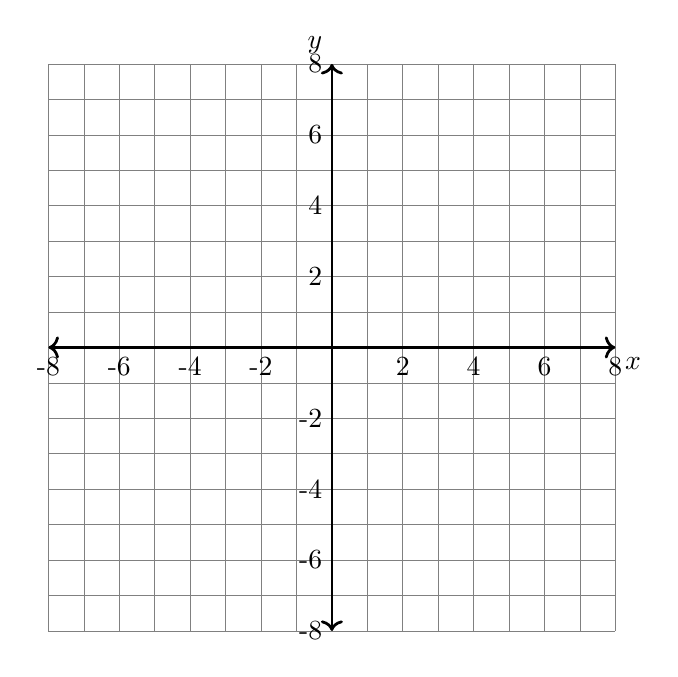
\begin{tikzpicture}[scale=0.45]
    \draw[step=1cm, gray, very thin] (-8,-8) grid (8,8);
    \draw[<->, line width=1pt] (-8,0) -- (8,0);
    \draw[<->, line width=1pt] (0,-8) -- (0,8);
    \foreach \x in {-8,-6,-4,-2,2,4,6,8}
    {
        \node[below] at (\x,0) {\x};
    }
    \foreach \y in {-8,-6,-4,-2,2,4,6,8}
    {
        \node[left] at (0,\y) {\y};
    }
    \node[below right] at (8,0) {$x$};
    \node[above left] at (0,8) {$y$};
\end{tikzpicture}
\end{center}
}

\begin{document}
\handwriting

\begin{center}
    \Large\textbf{\color{primaryblue}Module 1 Lesson 4\\Systems of Linear Equations in Two Variables and Applications} \\
    \vspace{0.2cm}
    \hrule
\end{center}

\section*{Objectives}

\begin{friendlyrule}{In this lesson, we will learn how to}
\begin{itemize}
    \item check whether an ordered pair solves a system of equations;
    \item solve a system by substitution;
    \item solve a system by elimination (addition);
    \item solve a system by graphing;
    \item classify systems as consistent/inconsistent and dependent/independent;
    \item apply systems of equations to real situations.
\end{itemize}
\end{friendlyrule}

\section*{1. Systems of Equations}

A \funhl{system of equations} is two or more equations considered together, for example

\[
\begin{cases}
5x-4y=20,\\
2x-3y=1.
\end{cases}
\]

The solution to a system is the ordered pair that makes \emph{both} equations true. A system may also have infinitely many solutions or no solution at all.

\begin{friendlyex}
Determine whether $(8,5)$ is a solution to the system above.
\end{friendlyex}

 

\begin{solutionbox}
Substitute $x=8$, $y=5$ into both equations.

\[
5(8)-4(5)=40-20=20.\ \checkmark
\]

\[
2(8)-3(5)=16-15=1.\ \checkmark
\]

Both equations are true, so $(8,5)$ \textbf{is} a solution to the system.
\end{solutionbox}

  

\section*{2. Solving by Substitution}

\begin{friendlyrule}{Substitution Method}
Solve one equation for one variable, then substitute that expression into the other equation. This produces a single equation in one variable, which can be solved.
\end{friendlyrule}

\begin{friendlyex}
Solve using the substitution method.
\begin{itemize}
    \item[(1)] $\begin{cases} x-y=5,\\ 2x-5y=1. \end{cases}$
    \item[(2)] $\begin{cases} 3x-y=-1,\\ 2x+y=11. \end{cases}$
\end{itemize}
\end{friendlyex}

 

\begin{solutionbox}
\textbf{(1)} From the first equation, $x=y+5$. Substitute into the second:

\[
2(y+5)-5y=1.
\]

\[
2y+10-5y=1.
\]

\[
-3y=-9\ \Longrightarrow\ y=3.
\]

Then $x=3+5=8$. The solution is $(8,3)$.

\textbf{(2)} From the first equation, $y=3x+1$. Substitute into the second:

\[
2x+(3x+1)=11.
\]

\[
5x+1=11\ \Longrightarrow\ x=2.
\]

Then $y=3(2)+1=7$. The solution is $(2,7)$.
\end{solutionbox}

  

\section*{3. Solving by Elimination (Addition)}

\begin{friendlyrule}{Elimination Method}
Combine the equations, possibly after multiplying one or both by a constant, so that one variable cancels when the equations are added.
\end{friendlyrule}

\begin{friendlyex}
Solve using the elimination method.
\begin{itemize}
    \item[(1)] $\begin{cases} 3x-2y=5,\\ x+y=5. \end{cases}$
    \item[(2)] $\begin{cases} 2x+6y=7,\\ 3x+9y=10. \end{cases}$
\end{itemize}
\end{friendlyex}

 

\begin{solutionbox}
\textbf{(1)} Multiply the second equation by $2$:

\[
2x+2y=10.
\]

Add to the first equation:

\[
(3x-2y)+(2x+2y)=5+10\ \Longrightarrow\ 5x=15\ \Longrightarrow\ x=3.
\]

From $x+y=5$: $y=5-3=2$. The solution is $(3,2)$.

\textbf{(2)} Multiply the first equation by $3$ and the second by $2$:

\[
6x+18y=21,
\]

\[
6x+18y=20.
\]

Subtracting gives

\[
0=1,
\]

which is \textbf{false}. This system has \textbf{no solution} --- the two lines are parallel.
\end{solutionbox}

  

\section*{4. Applications}

\begin{friendlyex}
A small business shipped $120$ packages one day. Customers are charged $\$3.50$ for each standard delivery package and $\$7.50$ for each express delivery package. Total shipping charges for the day were $\$596$. How many of each kind of package were shipped?
\end{friendlyex}

 

\begin{solutionbox}
Let $x$ be the number of standard packages and $y$ the number of express packages.

\[
x+y=120,
\]

\[
3.5x+7.5y=596.
\]

From the first equation, $x=120-y$. Substitute:

\[
3.5(120-y)+7.5y=596.
\]

\[
420-3.5y+7.5y=596.
\]

\[
420+4y=596\ \Longrightarrow\ 4y=176\ \Longrightarrow\ y=44.
\]

Then $x=120-44=76$.

There were $76$ standard packages and $44$ express packages.
\end{solutionbox}

  

\begin{friendlyex}
A bus company counted $32$ ticket receipts last Friday. A senior ticket costs $\$6.75$ and a regular ticket costs $\$10$. The driver collected $\$297.25$ total. Let $x$ be the number of senior tickets and $y$ the number of regular tickets. Find the ordered pair $(x,y)$.
\end{friendlyex}

 

\begin{solutionbox}
\[
x+y=32,
\]

\[
6.75x+10y=297.25.
\]

From the first equation, $y=32-x$. Substitute:

\[
6.75x+10(32-x)=297.25.
\]

\[
6.75x+320-10x=297.25.
\]

\[
-3.25x=-22.75\ \Longrightarrow\ x=7.
\]

Then $y=32-7=25$. The ordered pair is $(7,25)$.
\end{solutionbox}

  

\section*{5. The Graphical Method}

\begin{friendlyrule}{Graphical Method}
To solve a system by graphing, draw both lines and find the point(s) where they cross.
\end{friendlyrule}

\begin{friendlyex}
Solve by graphing:

\[
\begin{cases}
3x-2y=-7,\\
2x+y=7.
\end{cases}
\]
\end{friendlyex}

\begin{center}
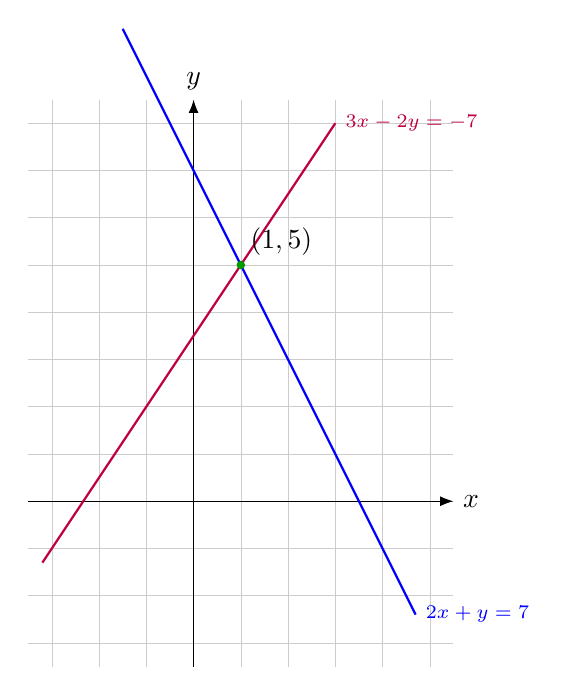
\begin{tikzpicture}[scale=0.6]
\draw[step=1, gray!40, very thin] (-3.5,-3.5) grid (5.5,8.5);
\draw[-{Latex}] (-3.5,0) -- (5.5,0) node[right] {$x$};
\draw[-{Latex}] (0,-3.5) -- (0,8.5) node[above] {$y$};
\draw[purple, thick, domain=-3.2:3, samples=2] plot (\x, {1.5*\x+3.5}) node[right] {\scriptsize $3x-2y=-7$};
\draw[blue, thick, domain=-1.5:4.7, samples=2] plot (\x, {-2*\x+7}) node[right] {\scriptsize $2x+y=7$};
\fill[green!60!black] (1,5) circle (0.09);
\node[above right] at (1,5) {$(1,5)$};
\end{tikzpicture}
\end{center}

 

\begin{solutionbox}
Graph the first equation. For the $x$-intercept, set $y=0$: $3x=-7 \Rightarrow x=-\frac73$. For the $y$-intercept, set $x=0$: $-2y=-7 \Rightarrow y=\frac72$.

Graph the second equation. For the $x$-intercept, set $y=0$: $2x=7 \Rightarrow x=\frac72$. For the $y$-intercept, set $x=0$: $y=7$.

Graphing both lines shows they intersect at

\[
(1,5).
\]

Check:

\[
3(1)-2(5)=3-10=-7.\ \checkmark
\]

\[
2(1)+5=2+5=7.\ \checkmark
\]
\end{solutionbox}

  

\section*{6. Classifying Systems}

\begin{friendlyrule}{Consistent or Inconsistent}
A system is \funhl{consistent} if it has one or more solutions --- the lines intersect or coincide. A system is \funhl{inconsistent} if it has no solution --- the lines are parallel.
\end{friendlyrule}

\begin{friendlyrule}{Dependent or Independent}
If a system represents the \emph{same} line, every point on that line satisfies both equations, so there are infinitely many solutions; we call the equations \funhl{dependent}. If the equations represent two \emph{different} lines, we call them \funhl{independent}.
\end{friendlyrule}

\section*{Summary}

\begin{friendlyrule}{Key Ideas}
\begin{itemize}
    \item A system's solution is the ordered pair satisfying every equation in the system.
    \item Substitution: solve for one variable, then substitute into the other equation.
    \item Elimination: multiply and add/subtract equations to cancel a variable.
    \item Graphing: the solution is the intersection point of the two lines.
    \item A false statement (like $0=1$) after elimination means no solution (inconsistent, parallel lines).
    \item A true statement (like $0=0$) after elimination means infinitely many solutions (dependent, same line).
\end{itemize}
\end{friendlyrule}

\end{document}
